\documentclass[12pt]{article}
\usepackage{amsmath}
\usepackage{amssymb}
\usepackage{geometry}
\usepackage{enumerate}
\usepackage{natbib}
\usepackage{float}%稳定图片位置
\usepackage{graphicx}%画图
\usepackage[english]{babel}
\usepackage{a4wide}
\usepackage{indentfirst}%缩进
\usepackage{enumerate}%加序号
\usepackage{multirow}%合并行
\title{\large UM-SJTU JOINT INSTITUTE\\Data Structures and Algorithms\\(VP281)\\\ \\\ \\\ \\\ \\\ \\\ \\\ \\\ \\\ \\\ \\\
Programming Assignment\\\ \\\ Programming Assignment Three\\\  Priority Queue and its Application \\\ \\\ \\\ \\\ \\\ }
\author{Name: Pan Chongdan\\ID: 516370910121}
\date{Date: \today}

\begin{document}
\maketitle
\newpage
\section{Introduction}
The programming assignment asks me to implement three priority queue including binary heap, unsorted heap and fibonacci heap. The goal is clear, use priority queue to find the shortest path from the source cell to the ending cell 
\par Second, thstudy the efficiency of different implementations. In lecture slides 13, professor gives a summary for the time complexity for binary heap and fibonacci heap.
\begin{figure}[H]
\centering
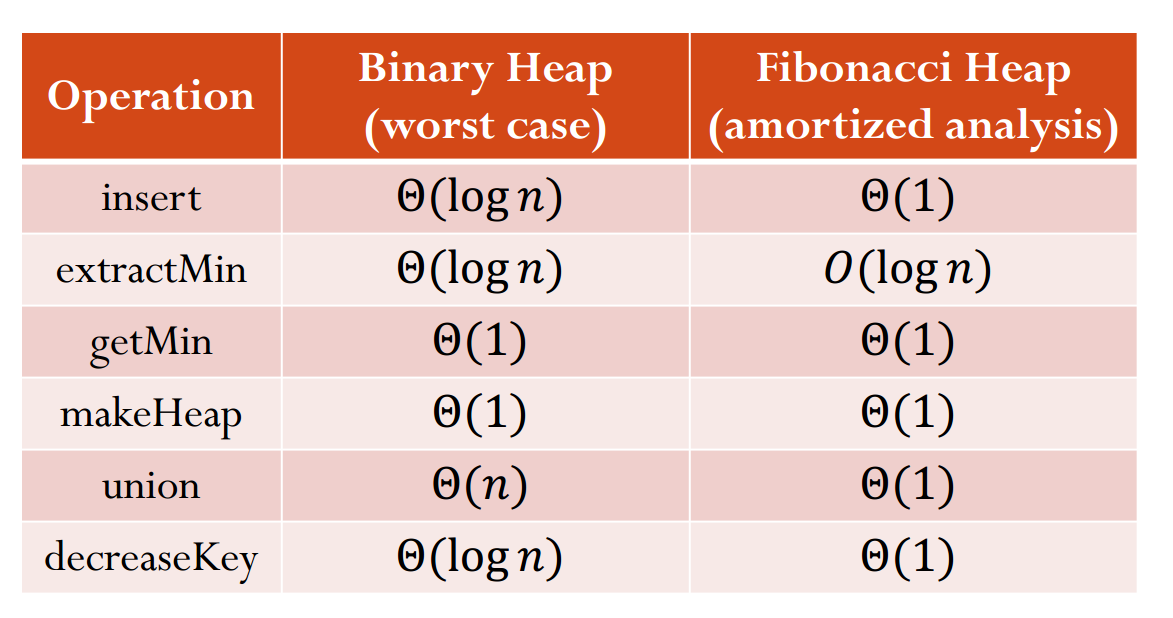
\includegraphics[scale=0.2]{P1.png}
\caption{Random Selection}
\end{figure}

\par However, we need to test the priority queue efficiency by ourselves, so I wrote a cpp file to print out the time required for each algorithm, which is included in appendix part.
\section{Result}
To test time efficiency, I used clock() function to get the time required. To get rid of other disturbing factor, I used to variable start and stop to get the time right before and after the sorting complete, then their difference is the time used. In my analysis, I get 7 set of data ,from which the map's length of side is 5,10,20,50,75,100,1000 and the size is the length's square.
\begin{table}[H]
\centering
\begin{tabular}{|c|c|c|c|c|c|c|c|}
\hline
map Size                 & 5    & 10   & 20     & 50    & 75    & 100  &1000
  \\ \hline
Binary Heap              &6.5e-5& 6.1e-5& 3.6e-4& 1.4e-3& 3.7e-3& 5.2e-3& 0.13      \\ \hline
Unsorted Heap        &5.5e-5& 6.3e-5& 4.2e-4& 2.6e-3& 1.1e-2& 1.9e-2& 2.1 \\ \hline
Fibonacci Heap     &1.2e-4& 1.3e-4& 1.7e-3& 4.7e-3& 1.9e-2& 2.9e-2& 0.92  \\ \hline
\end{tabular}
\end{table}
\section{Conclusion}
This chart is plot by matlab, showing the time efficiency of each algorithms compared to each other, and it has following characteristics.
\begin{figure}[H]
\centering
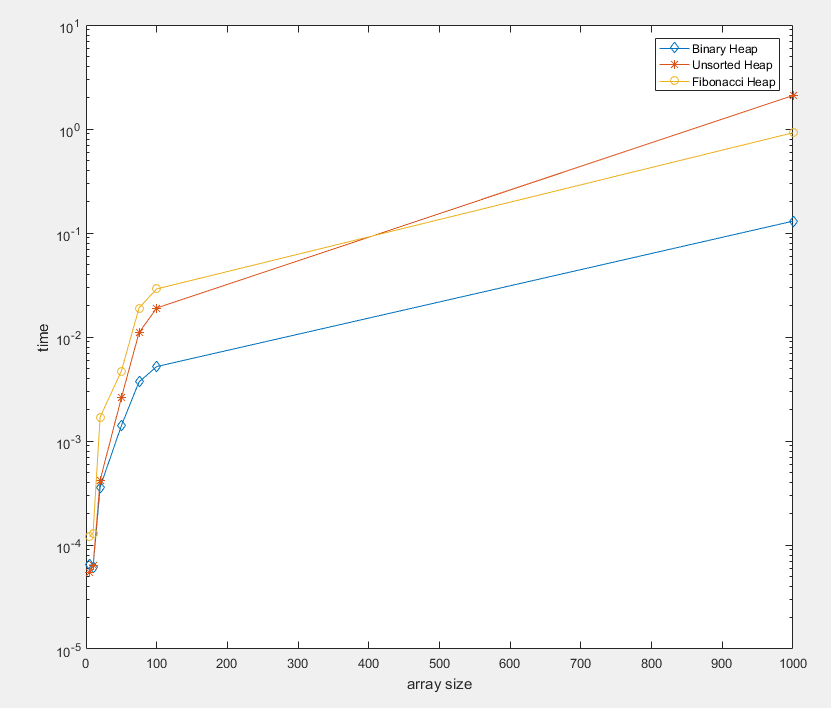
\includegraphics[scale=0.5]{P3.png}
\end{figure}
\begin{enumerate}
\item The average time required for each algorithm grows as the map grows bigger.
\item When the map is small, the time used for binary heap and unsorted heap is very close but binary have an advantage when the map is bigger as well as the Fibonacci.
\item Fibonacci heap always takes the longer time than Binary Heap, which is not reasonable, I think it's because it takes more time to use implement with list, but its time complexity is similar others from the picture
\end{enumerate}
\section{Appendix}
The appendix shows the cpp code for main project and time comparison.
The following part is for the main algorithm
\begin{figure}[H]
\centering
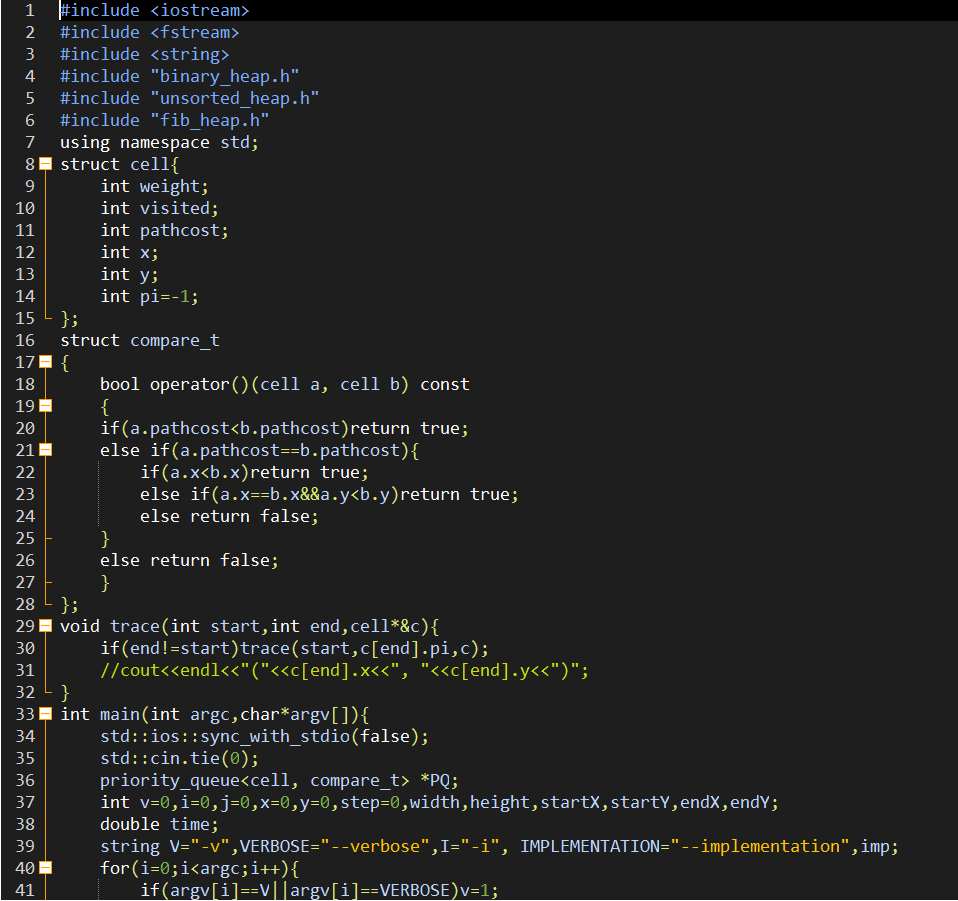
\includegraphics[scale=0.6]{P4.png}
\end{figure}
\begin{figure}[H]
\centering
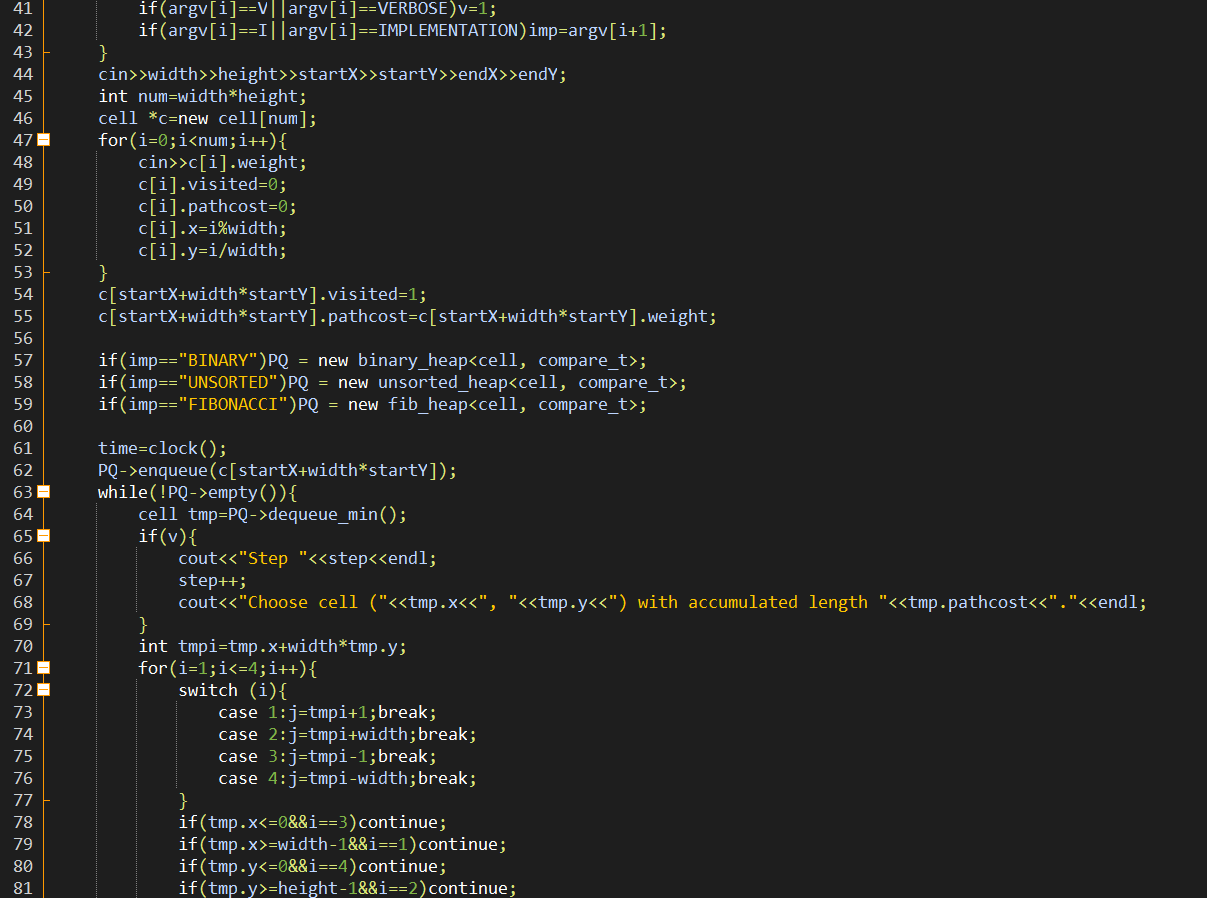
\includegraphics[scale=0.6]{P5.png}
\end{figure}
\begin{figure}[H]
\centering
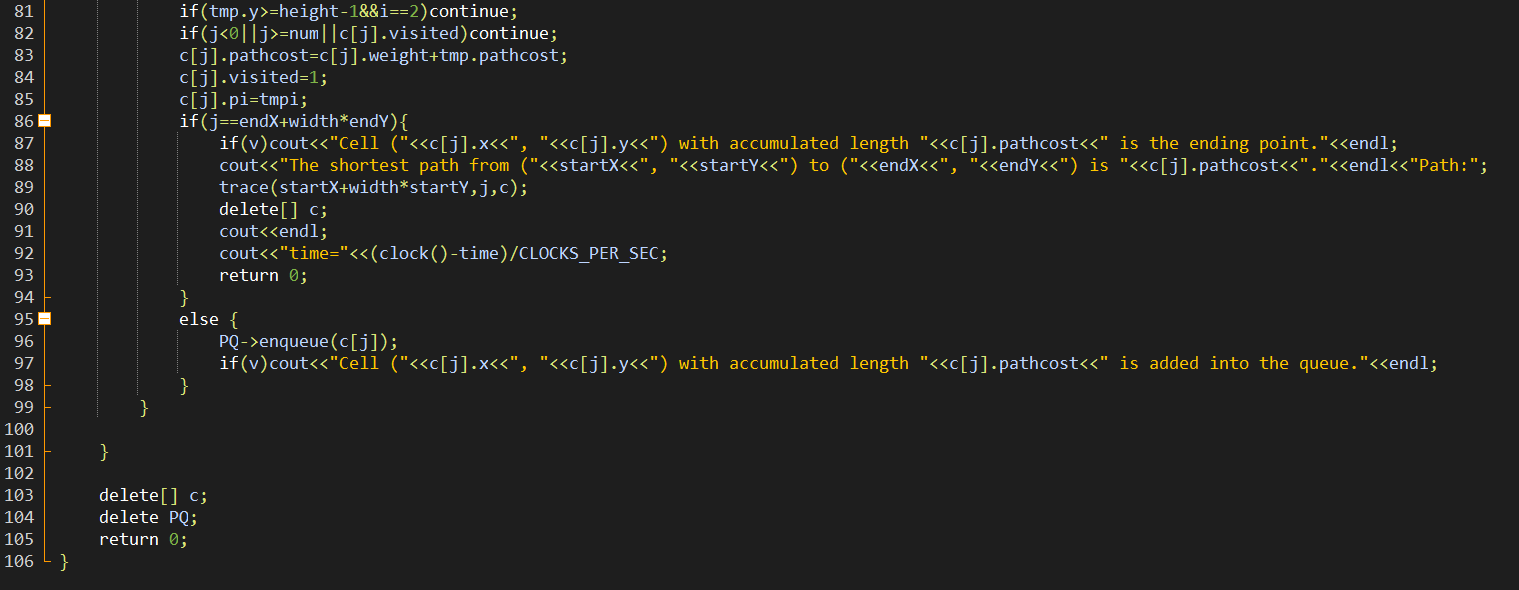
\includegraphics[scale=0.6]{P6.png}
\end{figure}
The following is for binary heap.
\begin{figure}[H]
\centering
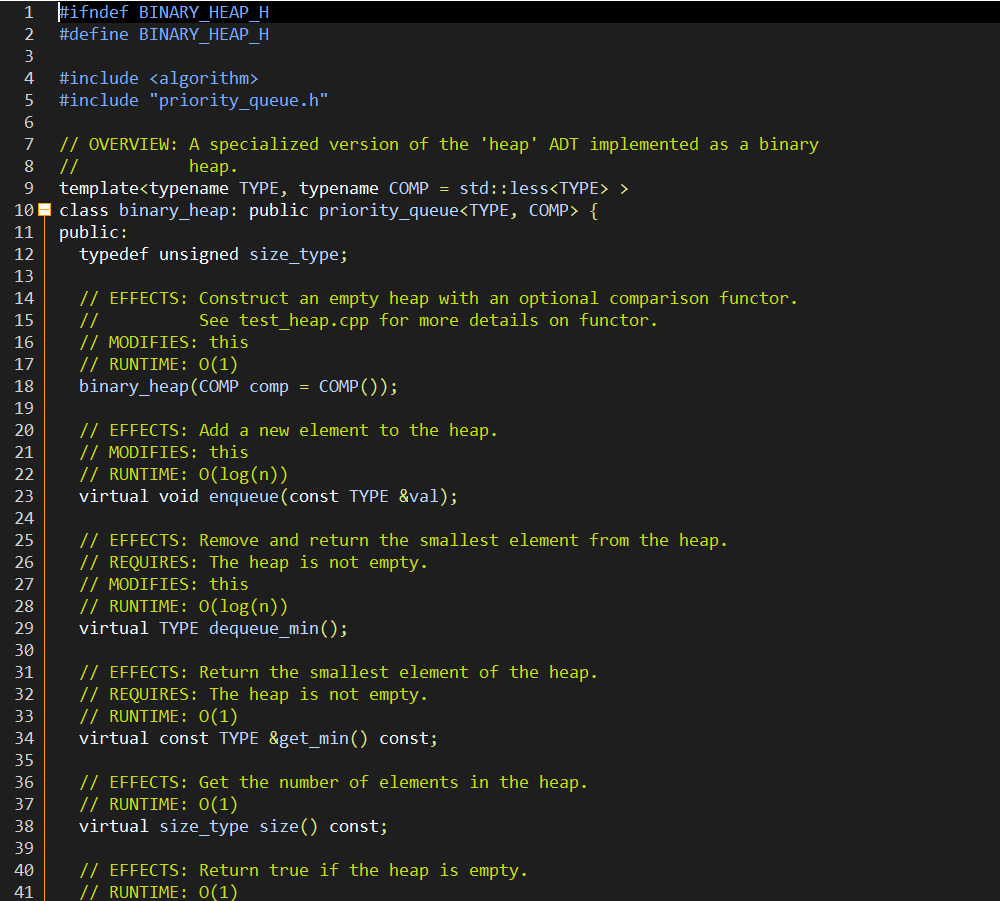
\includegraphics[scale=0.6]{P7.png}
\end{figure}
\begin{figure}[H]
\centering
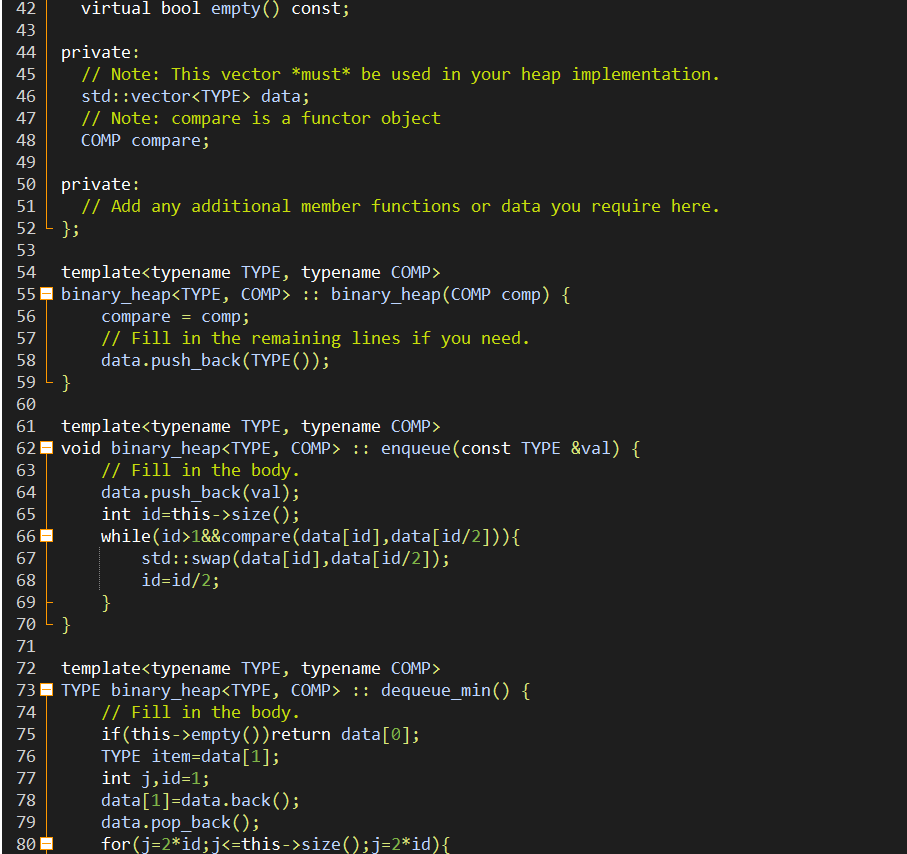
\includegraphics[scale=0.6]{P8.png}
\end{figure}
\begin{figure}[H]
\centering
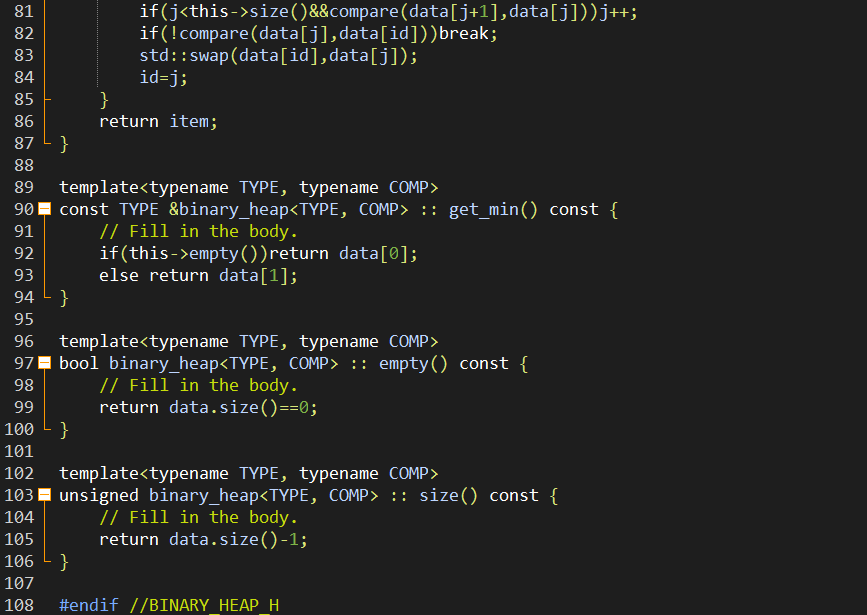
\includegraphics[scale=0.6]{P9.png}
\end{figure}
The following is for unsorted heap.
\begin{figure}[H]
\centering
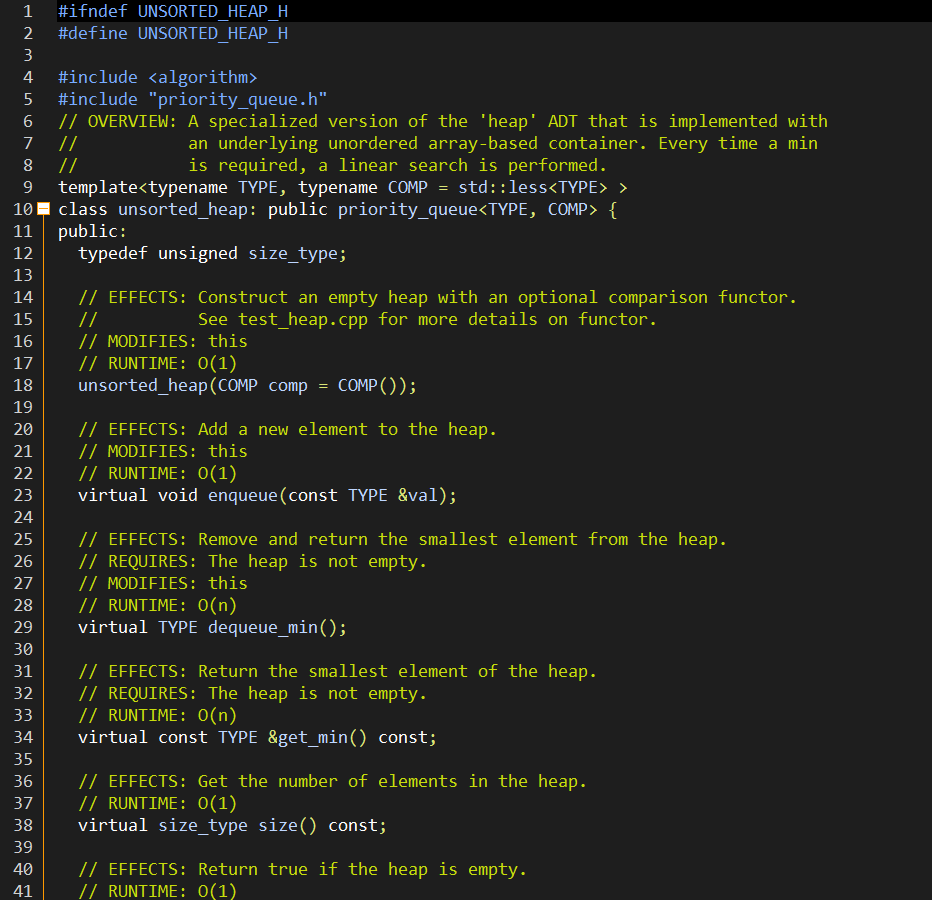
\includegraphics[scale=0.6]{P10.png}
\end{figure}
\begin{figure}[H]
\centering
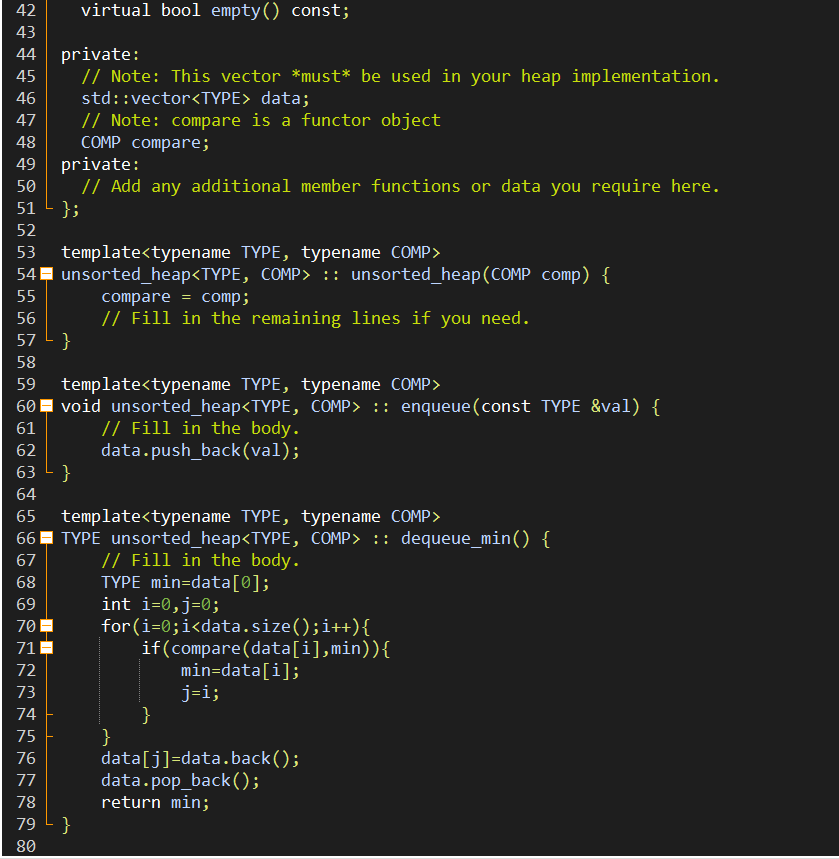
\includegraphics[scale=0.6]{P11.png}
\end{figure}
\begin{figure}[H]
\centering
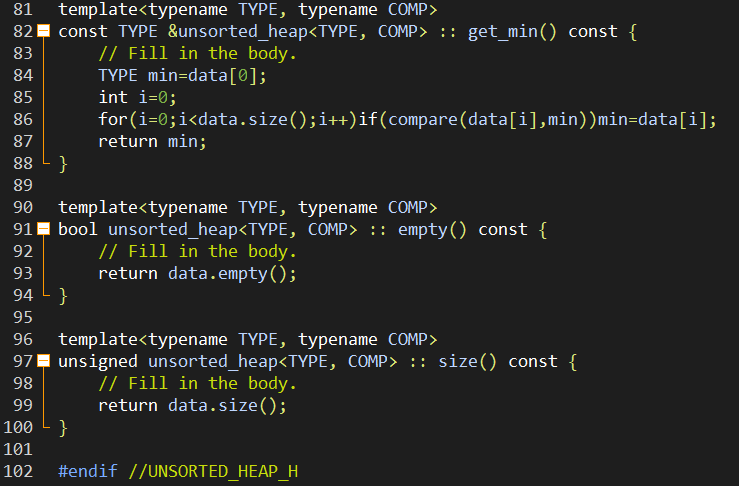
\includegraphics[scale=0.6]{P12.png}
\end{figure}
The following is for fibonacci heap.
\begin{figure}[H]
\centering
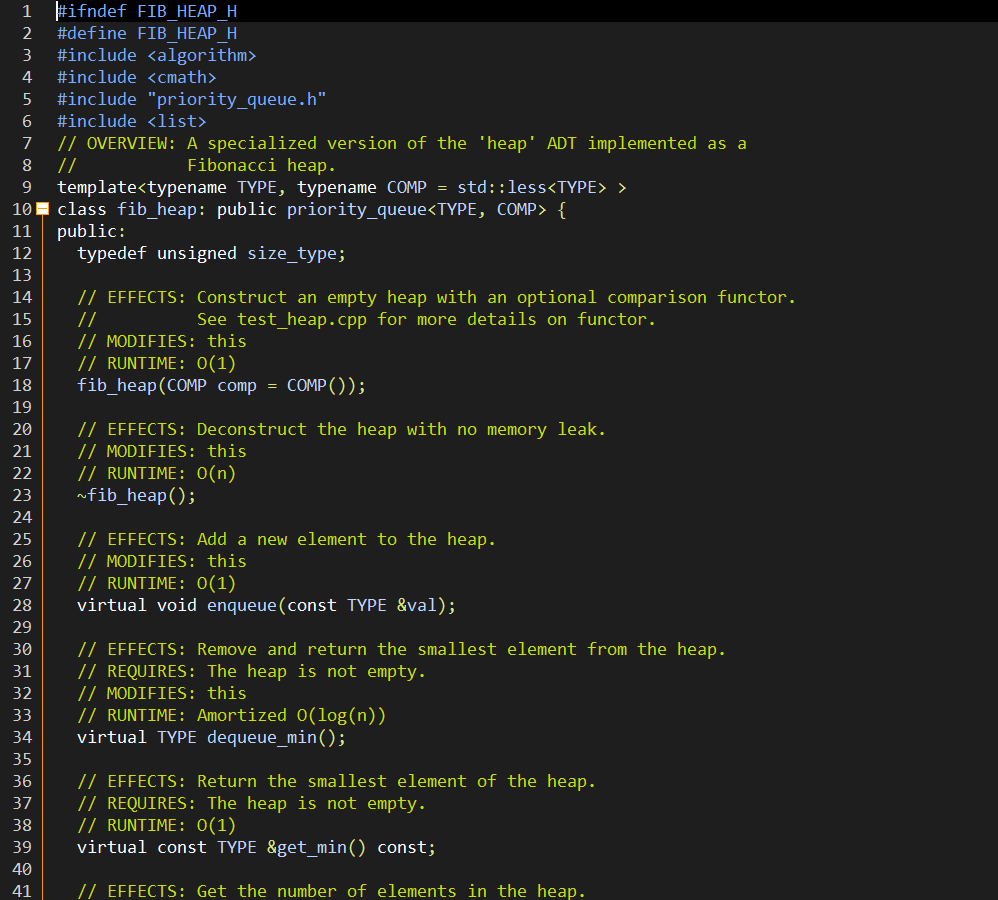
\includegraphics[scale=0.6]{P13.png}
\end{figure}
\begin{figure}[H]
\centering
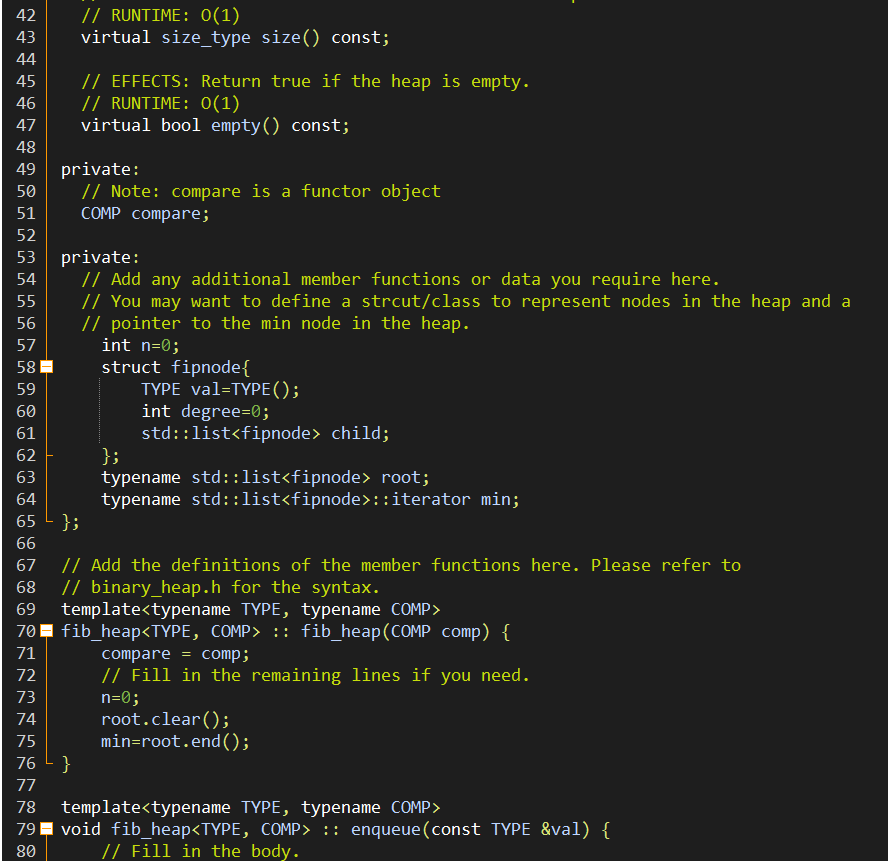
\includegraphics[scale=0.6]{P14.png}
\end{figure}
\begin{figure}[H]
\centering
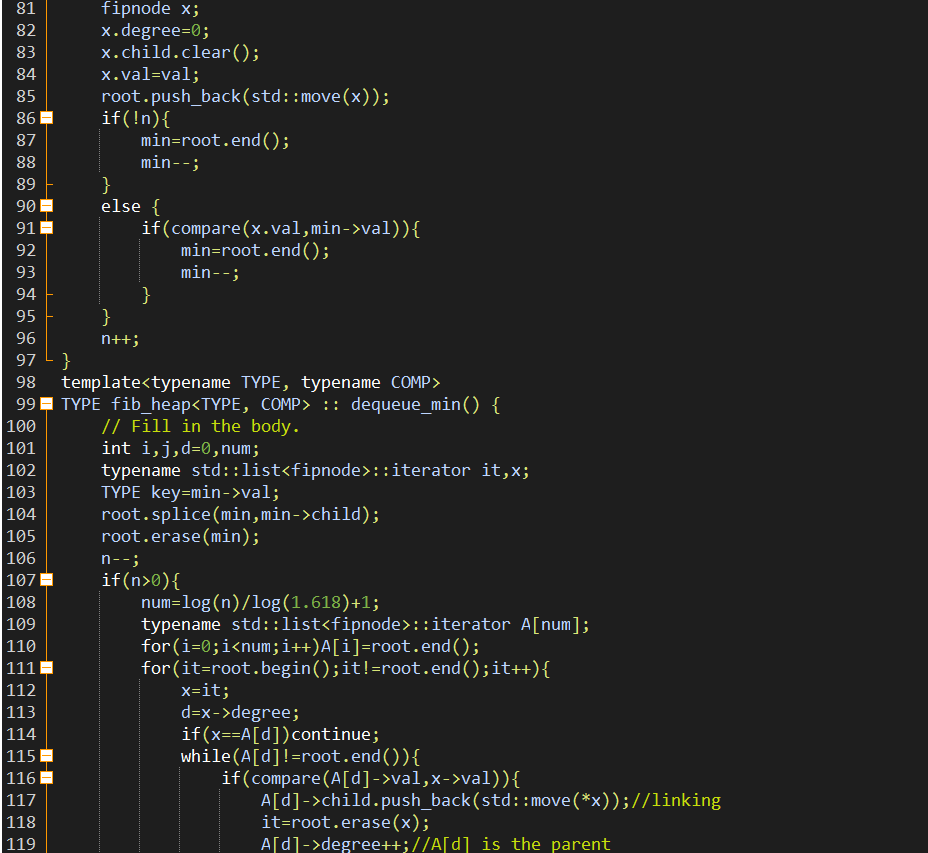
\includegraphics[scale=0.5]{P15.png}
\end{figure}
\begin{figure}[H]
\centering
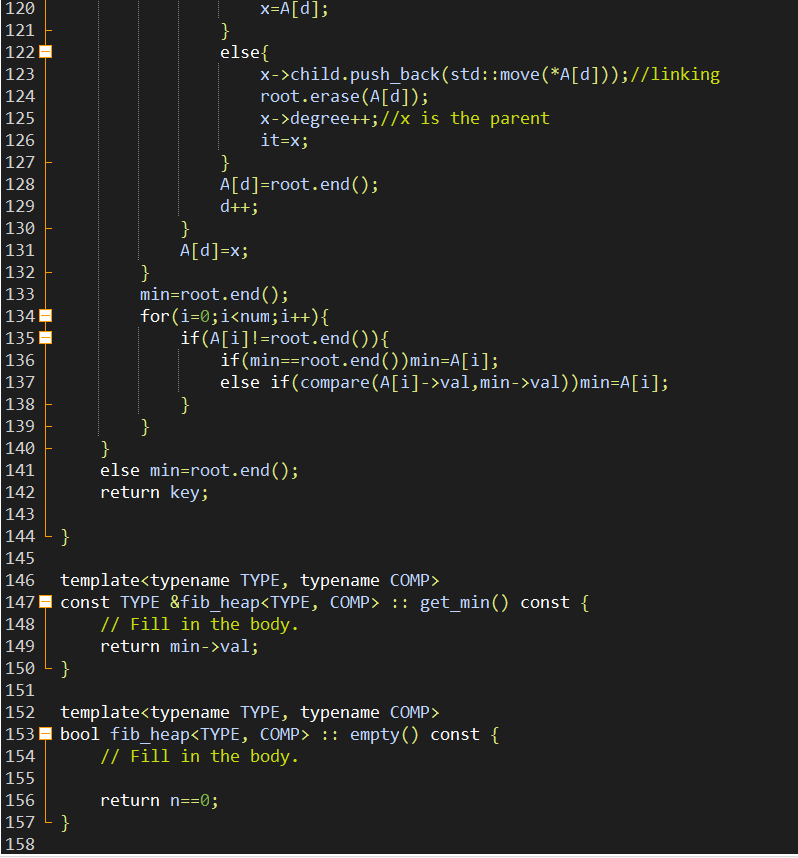
\includegraphics[scale=0.5]{P16.png}
\end{figure}
\begin{figure}[H]
\centering
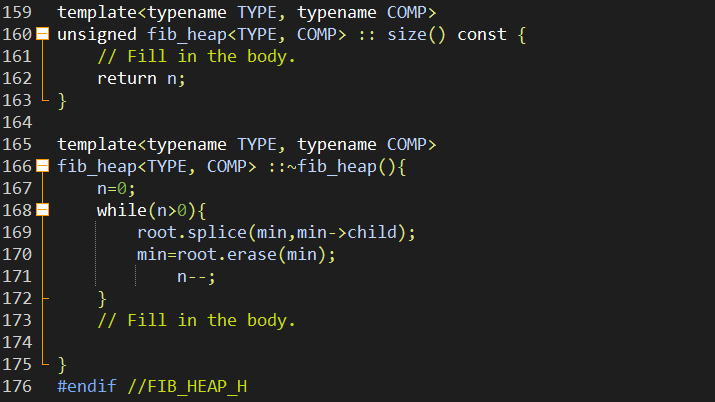
\includegraphics[scale=0.6]{P17.png}
\end{figure}
\end{document}